\section{Diskussion}
\label{sec:Diskussion}
Besonders augenfällig ist der plötzliche Sprung der aufgenommen Messwerte bei der Messung mit grünem Licht, siehe \autoref{fig:grun}.
Der Sprung kommt wahrscheinlich von einer Erschütterung der Messapparatur, welche mit sehr empfindlichen Koaxialkabeln aufgebaut ist.
In der \autoref{fig:gelba} wurden wegen des Sättigungswertes, der sich für hohe Beschleunigungsspannungen einsetzt, nicht alle Messwerte in die Ausgleichsrechnung einbezogen.
Der Beginn des linearen Zusammenhangs ist nur grob einschätzbar und durch eine leicht andere Wahl, könnten die errechneten Werte noch genauer oder ungenauer werden.
Die Werte an sich zeigen vor und nach dem Sprung das erwartete Verhalten, sodass ein weiterer Fehler durch die Geräte auszuschließen ist.
In der Auswertung fällt auf, dass die Messunsicherheiten der bestimmten Größen meist einen höheren Betrag haben als die eigentlichen Größen. 
Bei den Parameter der linearen Fits ist dies damit zu erklären, dass die gemessenen Werte in dem aufgetragenen Zusammenhang kein lineares Verhalten zeigt, also die Linearität eher erzwungen ist.
Die fällt besonders bei der \autoref{fig:b} auf, wobei hier die geringe Anzahl der Punkte zu beachten ist. 
Hier wurde mit dem Fit das Verhältnis $\frac{\symup{h}}{\symup{e}_0}$ ermittelt. 
\begin{align*}
    (\frac{\symup{h}}{\symup{e}_0})_{\text{theo}} &= \SI{4.135668e-15}{\volt\second}\\
    (\frac{\symup{h}}{\symup{e}_0})_{\text{exp}} &= \SI{3.533622(2056484)e-15}{\volt\second}
\end{align*} 
Damit beträgt die Abweichung vom Literaturwert $\SI{14.56}{\percent}$, welches in Anbetracht der anderen Werte ein recht gutes Ergebnis ist.

\newpage
\section{Anhang}
\begin{figure}
    \centering
    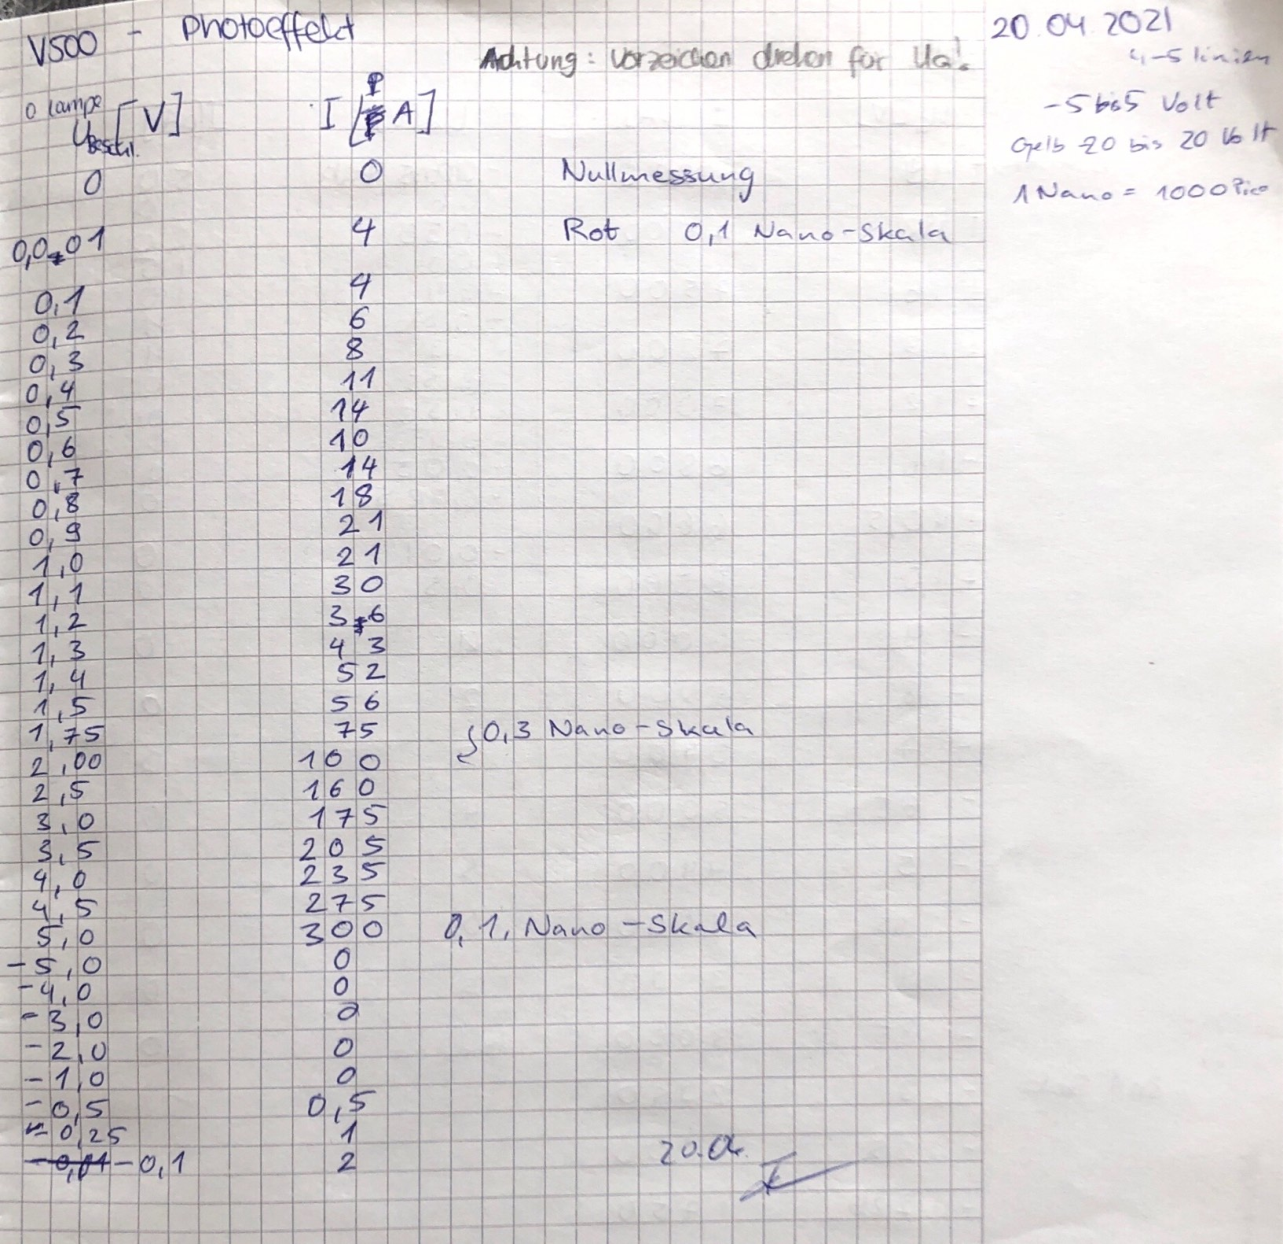
\includegraphics[width=\textwidth]{content/photorot.pdf}
\end{figure}
\begin{figure}
    \centering
    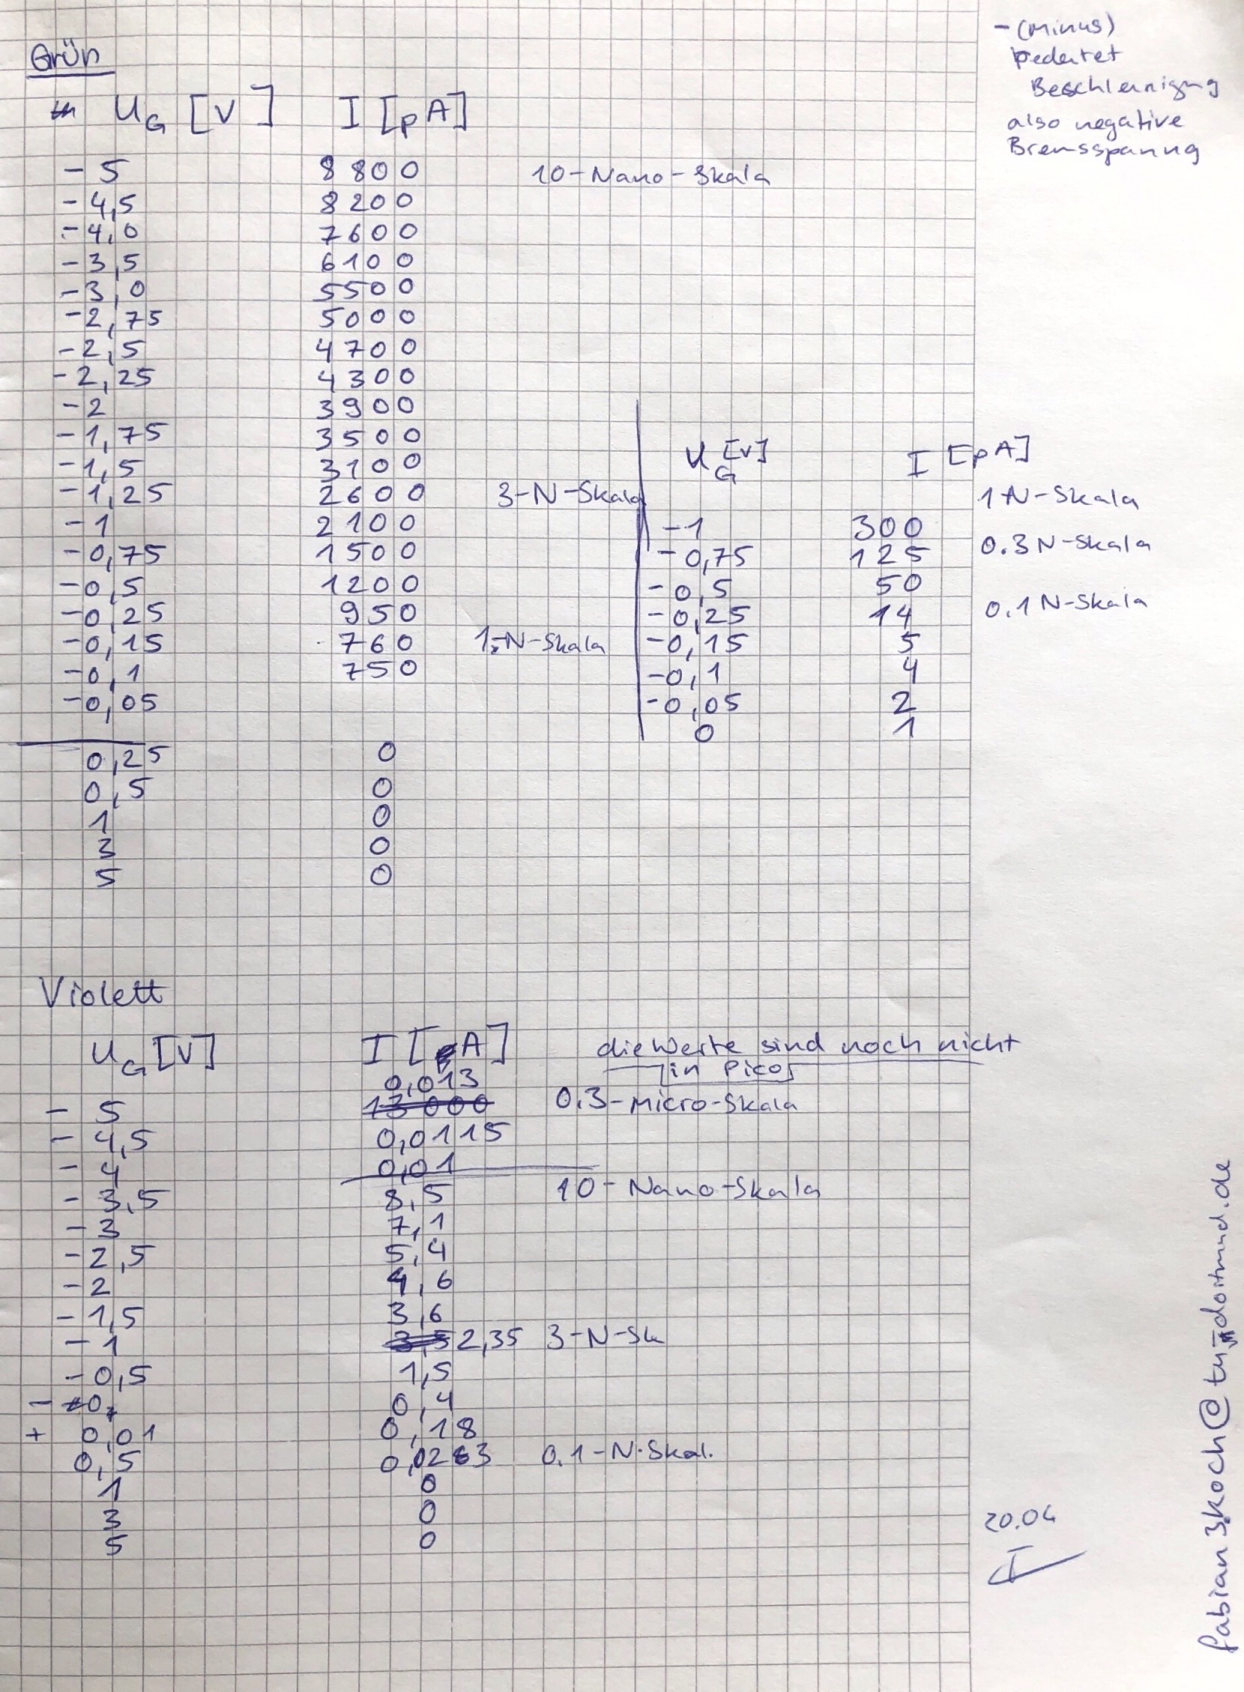
\includegraphics[width=\textwidth]{content/photogrunvio.pdf}
\end{figure}
\begin{figure}
    \centering
    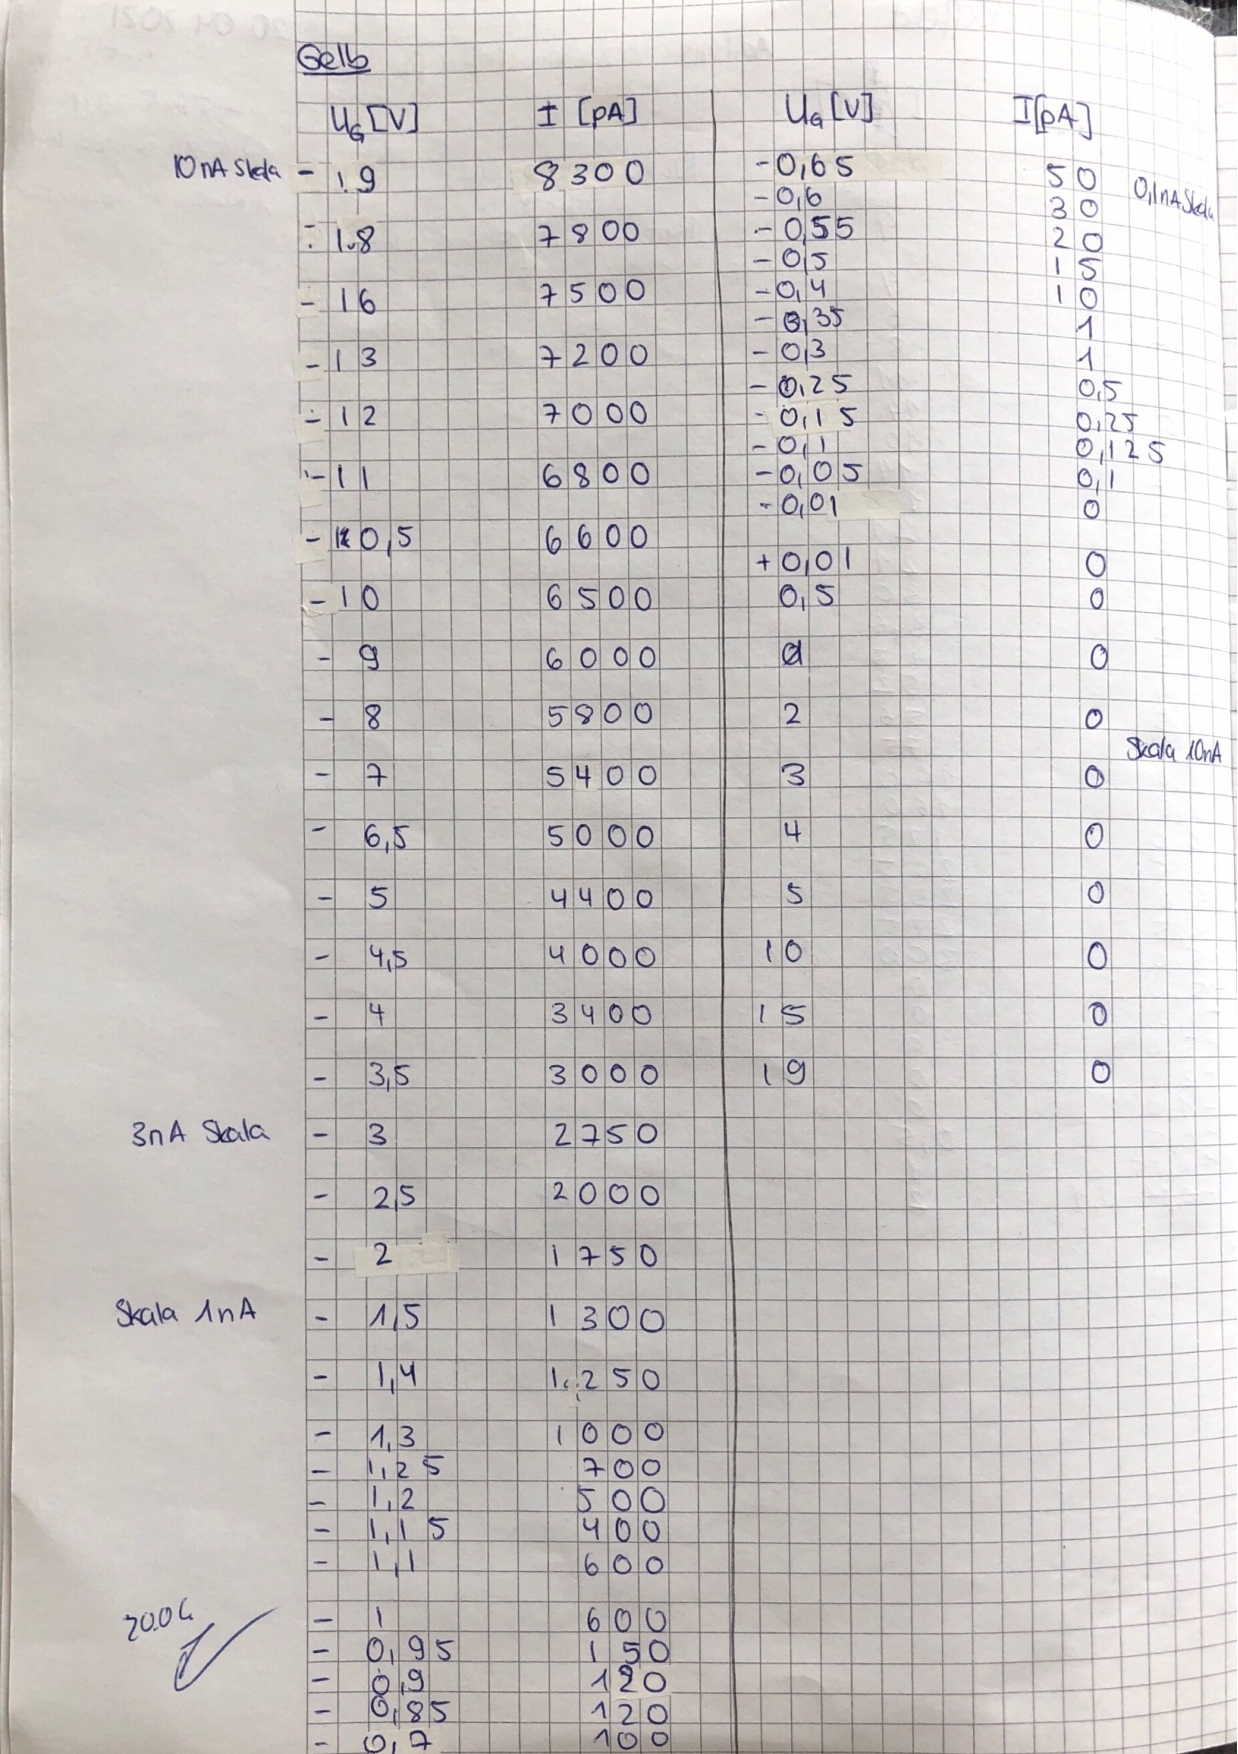
\includegraphics[width=\textwidth]{content/photogelb.pdf}
\end{figure}